\documentclass{beamer}
\newcommand{\myfont}{\rmfamily\normalsize\upshape\mdseries}
\newcommand{\degree}{^\circ}
\title{\sffamily Review VI(Slides 350 - 413)}
\subtitle{\textbf{Graph Theory}}
\institute[UM-SJTU JI]{University of Michigan-Shanghai Jiao Tong University Joint Institute}
\author{HamHam}
\usepackage{graphicx}
\usepackage{picinpar}
\usepackage{indentfirst}
\usepackage{chemformula}
\usepackage{geometry}
\usepackage{subfigure}
\usepackage{appendix}
\usepackage{amsfonts}
\usepackage{enumerate}
\usepackage{float}
\usepackage{geometry}
\usepackage{latexsym}
\usepackage{listings}
\usepackage{multicol,multirow,multido}
\usepackage{tabularx}
\usepackage{ulem}
\usepackage{tikz}
\usepackage{xcolor}
\usepackage{cite}
\usepackage{setspace}
\usepackage{hyperref}
\usepackage{textpos}
\usepackage{booktabs}
\usepackage{diagbox}
\usepackage{listings}
\usepackage{graphics}
\usepackage{upgreek}
\usepackage{JI_MathCourse_Notations}
\usepackage{mathrsfs}
\usepackage[thicklines]{cancel}
%定义绘制椭圆的命令,带有四个参数
%第一个参数:椭圆位置的横坐标
%第二、三参数:椭圆x位置的半径、y位置的半径
%第四个参数:填充的透明度
\def\drawell#1#2#3#4{
	\draw[draw=black,fill=gray,fill opacity=#4,line width=3pt] 
	(#1,0) circle [x radius=#2, y radius=#3];}

%\usepackage{ctex} %插入中文
%\ctexset{today=old}

\newcommand{\mydef}[1]{\sffamily\blue{#1}\myfont\\} %for define
\newcommand{\mysol}{\yellow{Solution:}\\}
\usetheme[dove]{Boadilla}
\usecolortheme{dolphin}
\useoutertheme{miniframes}
\begin{document}
    \usebackgroundtemplate{\tikz\node[opacity=0.25]{
    
\includegraphics[width=\paperwidth,
    height=\paperheight]{hamster.jpg}
    };}
\begin{titlepage}
    \begin{center}
        VE203 - Discrete Mathmatics 
    \end{center}
\end{titlepage}
\myfont
\newcommand{\binomial}[2]{\begin{pmatrix} {#1}\\{#2}	\end{pmatrix}}
\newcommand{\green}[1]{\textcolor[rgb]{0.3,0.6,0}{#1}}

\section{Basics}
\begin{frame}
    \frametitle{Terminology}
    Some notations, properties, operations\dots
    \begin{itemize}
        \item vertex set $V$
        \item edge set $E$
        \item adjacent
        \item loop
        \item parallel
        \item simple graph
        \item isomorphism  $G\cong H$
        \item complment $\conj{G}$
        \item degree $\deg(v)$
        \item distance $\dist{u}{v}$
    \end{itemize}
    

\end{frame}
\begin{frame}
    \frametitle{Standard Graphs}
    \hh You should  remember  both the \green{names} and  the \blue{notations}. Let's see them in 
    \red{Mathematica}!
    \begin{itemize}
        \item Complete Graph $K_n$
        \item Clique
        \item Path $P_n$
        \item Cycle Graph $C_n$
        \item Bipartite Graphs $K_{m,n}$
        \item *Wheel Graph $W_n$
        \item *Qubic Graph $Q_n$
    \end{itemize}
    \begin{block}{Attention: null graph}
        \hh $G=\(V,\varnothing\)$ or $G=\(\varnothing,\varnothing\)$ ?
    \end{block}

\end{frame}
\begin{frame}
    \frametitle{Exercise}
    
    \hh 1. The complement of a simple graph $G = (V, E\,)$ is given by $G\,^c = (V, E\,^c
    )$, where $E\,^c = V \times V ~\cut~ E$, i.e., the
    complement has the same vertex set and an edge is in $E\,^c$
    if and only if it is not in $E$. A graph $G$ is said to be
    \blue{\textit{self-complementary}} if $G$ is isomorphic to $G\,^c$
    .\\ \vv
    \begin{itemize}
        \item[i)] Show that a self-complementary graph must have either $4m$ or $4m + 1$ vertices, $m\in\bN$.
        \item[ii)] Find all self-complementary graphs with 8 or fewer vertices.
    \end{itemize}
    \vv
    (Taken from Ve203 FA2020 Assignment10)
\end{frame}
\begin{frame}
    \frametitle{The Handshaking Theorem}
    Undirected graph:
    $$2|E\,| = \sum_{v\in V}\deg(v)$$
    Directed graph:
    $$|E\,| = \sum_{v\in V} \deg^+ (v) = \sum_{v\in V} \deg^- (v)$$
    \green{Remark:}\\
    \begin{itemize}
        \item A vertex is said to be \textbf{\green{isolated}} if it has degree zero.
        \item A vertex is said to be \textbf{\green{pendant}} if it has degree one.
        \item $\deg^+(v)$: in-degree of a vertex v
        \item $\deg^-(v)$: out-degree of a vertex v
    \end{itemize}
\end{frame}
\section{Conectivity}

\begin{frame}
    \frametitle{Walks and Connectivity}
    \mydef{Definition}
    \hh A \blue{walk} $W$ in $G$ is a sequence of vertices
    \green{$\{v_i\}^n_{i=0}$} and edges 
    \green{$\{e_i\}^n_{i=1}$} so that $e_i$
    is incident with $v_{i-1}$ and $v_i$. 
    \begin{itemize}
        \item $W$ is 
        called \textbf{closed} if $v_n=v_0$
        \item The \textbf{length} of $W$ is its number
        of edges $n$
        \item $G $ is connected if $\forall u,v \in V\(G\)$,
        there is a walk from $u$ to $v$
    \end{itemize} 
\end{frame}

\begin{frame}
    \frametitle{Exercise}
    2. Judge whether the following statements are true or false.
    \begin{itemize}
        \item  A walk must be a path or cycle.
        \item If there is a walk from $u$ to $v$, there is also such a path.
        \item $G$ is disconnected if\mbox{f} there is a partition $\{X, Y\}$ of $V\(G\)$ such that
        no edge has an \textbf{\green{end}} in $X$ and an end in $Y$.
        \item For two connected subgraphs $H_1, H_2 \subset G$ that $V(H_1) \cap V(H_2) \not= \varnothing $,
        $H_1 \cup H_2 := \(V(H_1) \cup V(H_1), E(H_1) \cup E(H_1)\)$ is connected.
        
    \end{itemize}

\end{frame}
\begin{frame}
    \frametitle{Components}
    \mydef{Definition}
    \hh A component of a graph $G$ is a 
    \textbf{maximal connected subgraph} in
    $G$. In other words, it is not contained in any other connected
    subgraphs. 
    \\ \hh The number of components of $G$ is denoted as
    $\comp{G}$.
    \\
    \mydef{Theorem}
    \hh Every vertex is a \textbf{unique} component.
    \begin{block}{Note}
        \hh If a graph $G$ isn't connected, it may be useful
        to consider its components.
    \end{block}
\end{frame}
\begin{frame}
    \frametitle{Exercise}
    3. Show that a simple graph $G:=\(V,E\,\)$ with $|V\,|=n,n\geq 2$ is 
    connected if $|E\,| >(n-1)(n-2)/2$.
    \pause 
    \\\vs{3em}
    \begin{block}{Hints}
        \begin{itemize}
            \item Consider components $V_1, V_2, \dots, V_k$...
            \item $K_{n-1}$ could only have at most $\binomial{n-1}{2}$ edges.
            \item Alternatively, does induction help?
        \end{itemize}
    \end{block}
    \hh 
\end{frame}
\begin{frame}
    \frametitle{Cuts}
    \mydef{Definition(substraction)}
    \hh Given $G = \(V, E\,\)$, $S \subset E$, $X \subset V$, 
    then $G - S := \(V, E~\cut~S\)$ and
    $G - X := (V~\cut~ X, \{e \in E : e \text{ not incident with }x \in X\})$.
    \\ \vv
    \mydef{Definition}
    \begin{itemize}
        \item $e \in E$ is a \textbf{cut-edge} or \textbf{bridge} 
        if no cycle contains $e$
        \item $v \in V $ is a \textbf{cut-vertex} if 
         $\comp{G-v} > \comp{G}$
    \end{itemize}
    \green{What happens when we delete an edge or vertex?}
    \begin{itemize}
        \item If $e$ is a cut-edge, $\comp{G-e}=\comp{G}+1$
        \item If $e$ is not, $\comp{G-e}=\comp{G}$
        \item Further, $\comp{G-v} \leq \comp{G} + \deg\(v\) -1$
    \end{itemize}
    \green{Induced subgraph}
    \\ \hh \red{Please remember to delete both the vertexes and the edges!}
\end{frame}
\newcommand{\sweat}{
\includegraphics[width=0.03\textwidth]{sweat.png}}
\begin{frame}
    \frametitle{Exercise}
    \green{The followings was going to appear in the exam}.\\
    4. Given a graph $G$ shown as follows:
    \begin{center}
        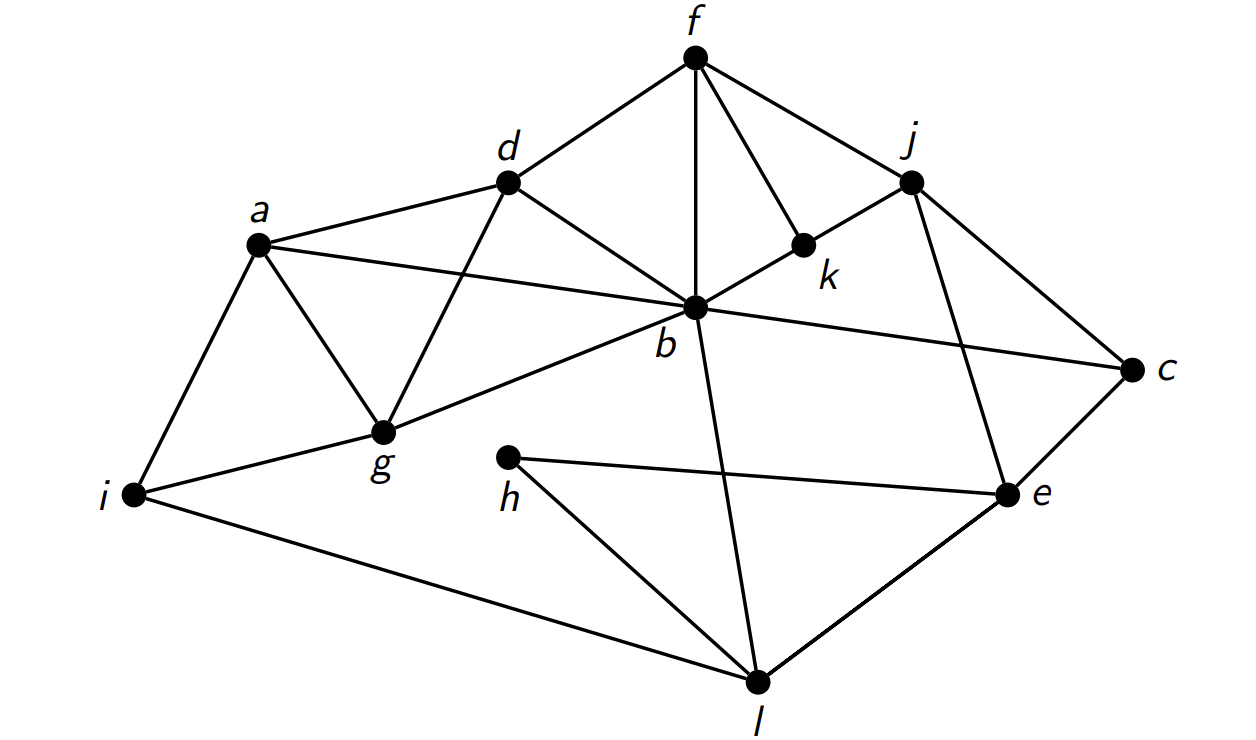
\includegraphics[width=0.56\textwidth]{graph.png}
    \end{center}
    List the corresponding vertices or edges of $G$ for the following:
    \begin{itemize}
        \item Find a clique of size 4/ size 5 if possible
        \item Find a induced cycle of size 4 / size 5 if possible
        \item Find a maximal matching that is \textbf{NOT} maximum.
    \end{itemize}
\end{frame}
\section{Matching}
\begin{frame}{Bipartation \& Matching}
    \mydef{Theorem}
    For every graph $G$, the following are equivalent:
    \begin{itemize}
        \item $G$ is bipartite
        \item $G$ has no cyle of odd length
        \item $G$ has no closed walk of odd length
        \item $G$ has no induced cycle of odd length.
    \end{itemize}
    \vv 
    \mydef{Compare and Contrast}
    \begin{itemize}
        \item Maximal chain/ maximum chain
        \item Maximal matching/maximum matching
    \end{itemize}

\end{frame}
\begin{frame}
    \frametitle{Hall's Theorem}
    \hh Let $G$ be a bipartite graph with bipartation $\(A, B\)$. There exists a
    matching covering $A$ if\mbox{f} there does not exist $X \subset A$ with $|N\(X\)| < |X|$.
    \\ \vv
    \green{Exercise}
    \\ \hh  Given $m$ (not necessarily
    distinct) finite sets $S_1, S_2, \dots, S_m$, there exists a list of distinct elements $x_1, x_2, \dots, x_m$ such that
    $x_i \in S_i$
    for all $i = 1, 2, \dots, m$ iff \textbf{Hall's condition} holds. 
    State \textbf{Hall's condition} in this context.
    \\ \vv
    \pause
    \mysol
        \hh For every $k=1,2,\dots,m$, the union of 
        any $k$ sets has at least $k$ elements, that is 
        $$|\bigcup_{i\in I} S_i|\geq |I\,| \text{ for all } I \subset \{1,\dots,m\}$$
\end{frame}

\section{Trees}
\begin{frame}
    \frametitle{Trees}
    Recall:
    \begin{itemize}
        \item forest
        \item tree 
        \item leaf 
    \end{itemize}
    \begin{block}{Exercise}
        \hh Let $T$ be a tree, $v$ be its leaf. 
        Judge whether the following statements are correct or not :
        \begin{enumerate}
            \item $\comp{G\,} = |V\(G\,\)| - |E\(G\,\)|$
            \item $|V\(T\,\)|=|E\(T\,\)|+1$
            \item $T-v$ is a tree
        \end{enumerate}
    \end{block}
\end{frame}
\begin{frame}
    \frametitle{What's more?}
    \begin{itemize}
        \item Ramsey Number
        \item Hungarian Algorithm
        \item Union-Find-set
        \item Dynamic Programming on Trees
        \item ...
    \end{itemize}
    

\end{frame}
\section{End}
\begin{frame}
    \frametitle{Reference}

    \begin{itemize}
        \item Homework exercises from 2020-Fall-Ve203
        \item Exercises/graphics from 2021-Fall-Ve203 TA Xue Runze
    \end{itemize}

\end{frame}
\begin{frame}
    \centering
    \Huge{$\mathcal{THANKS}$!}
\end{frame}

\end{document}